\documentclass[%
 reprint,
 amsmath,amssymb,
 aps,
 10pt
]{revtex4-2}
\usepackage{graphicx}% Include figure files
\usepackage[version=4]{mhchem}
\usepackage{dcolumn}% Align table columns on decimal point
\usepackage{bm}% bold math
\usepackage{siunitx}
\usepackage{lmodern}
\showthe\columnwidth
\usepackage[mathlines]{lineno}% Enable numbering of text and display math
\begin{document}
\begin{abstract}
	  Materials not usually associated with being magnetic can demonstrate magnetic susceptibility at room temperature. These materials are often called paramagnetic or diamagnetic. This experiment acts as a study into 16 different such materials. For each material it's magnetic susceptibility was calculated this also gave information as to whether the material was paramagnetic or diamagnetic. Understanding diamagnetic and paramagnetic substances is important because it relates to how quantum mechanics can have effects on bulk materials.
\end{abstract}
\preprint{AAPM/123-QED}
\title[title]{Forces on Materials within Magnetic Fields}
\author{Parker Wise$^{1}$ and Lucciana Cáceres$^{1}$\\$^{1}$University of Kansas}
\date{February 2025}
\maketitle
\showthe\textwidth
\section{Introduction}
The change of mass of a material in a magnetic field can be modeled as,
\begin{equation}
	\Delta m = \frac{\chi A}{2\mu_0 g}\left(B_\mathrm{top}^2-B_\mathrm{bottom}^2\right),
	\label{mass}
\end{equation}
where $\chi$ is the magnetic susceptibility, $\mu_0$ is the magnetic permeability of free space, $g$ is the average gravitational field at the surface of the Earth, and A is the cross sectional area of the material. This equation can be rearranged to solve for $\chi$ as,
\begin{equation}
	\chi = \frac{2\mu_0 g\Delta m}{A}\left(B_\mathrm{top}^2-B_\mathrm{bottom}^2\right)^{-1}.
	\label{chi}
\end{equation}
Equation \ref{chi} will be used in order to calculate $\chi$ for all of our materials. Materials with $\chi > 0$ are paramagnetic and materials where $\chi < 0$ are diamagnetic.
\section{Methods}
\begin{figure*}
	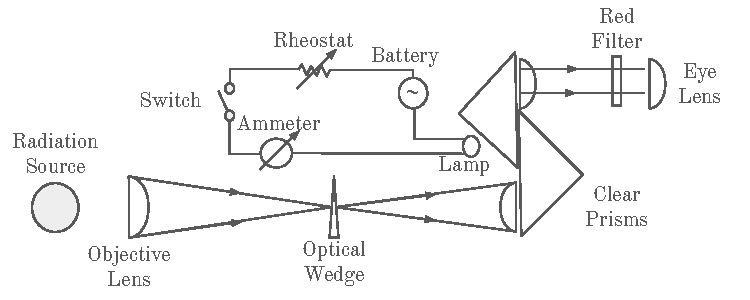
\includegraphics{setup.pdf}
	\caption{\label{app} The apparatus used for this experiment. The whole experiment was conducted on top of a scale. There was a clear platform upon which the magnet was placed. Tested materials were suspended within the magnetic field using a lifter rod.}
\end{figure*}
The apparatus for this experiment can be seen in figure \ref{app}. This experiment was conducted by measuring the affect that several materials had on a magnet. Due to the properties of the materials, when they entered the field of the magnet, a force was applied both to the magnet as well as the material. This force applied to the magnet was then measured on the scale and recorded. 
\par
Measurements were taken several times for each material at one of three positions. The first position was where the material was far away from the magnetic field and little force was measured on the magnet. The other two measurements were taken with half of the substances within the magnetic field. One with the upper half in the field, and one with the lower half in the magnetic field. The field between the magnets has a strength of $0.4$ T.
\par
From these mass measurements we were able to find two $\Delta m$ values, one where $\left(B_\mathrm{top}^2-B_\mathrm{bottom}^2\right = 0.4^2$ T, and another where $\left(B_\mathrm{top}^2-B_\mathrm{bottom}^2\right) = -0.4^2$ T. These values of $\Delta m$ where used to calculate $\chi$.
\section{Results}
\begin{figure*}
	\includegraphics{plots.pdf}
	\caption{\label{result-fig} This graph shows all 16 of the materials tested. There are two points on each graph, at $\pm 0.4^2$ T. The x-axis markings were omitted to conserve space, since they are all the same. Similarly $(NH4)2Fe(SO4)2(6H2O)$ and $NH4Fe(SO4)2(12H2O)$ were abbreviated. The magnetic field value is contrasted with the change in mass that has occurred. The slope of this of the line in each of the graphs corresponds to $\chi$ for that material.} 
\end{figure*}
In figure \ref{result-fig} a graph is shown for each of the 16 tested materials. The slope of these subplots corresponds to $\chi$ and was solved for using equation \ref{chi}. These calculated values and their propagated uncertainty can be seen in table \ref{table}. From this table we are able to gather which materials are paramagnetic and diamagnetic.
\begin{table*}
\centering
	\begin{tabular}{cccc}
		\hline
		Chemical &  $\Delta m_\mathrm{low}$ & $\chi^\mathrm{(mks)}$&$\pm \sigma_{\chi}$\\
		&g&$10^{-6}$&$10^{-6}$\\
		\hline \hline

$\ce{Cu}$ & -0.005 & -7.6969 & 13.9397\\
$\ce{Al}$ & 0.013 & 20.0119 & 12.0229\\
$\ce{Ti}$ & 0.128 & 197.041 & 9.85684\\
$\ce{Bi}$ & 0.259 & 398.7 & 729.706\\
$\ce{Co}$ & 0.196 & 301.719 & 10.3265\\
$\ce{C}$ & -0.057 & -87.7447 & 6.34703\\
$\ce{Nd2O3}$ & 1.838 & 2829.38 & 83.2548\\
$\ce{Gd2O3}$ & 2.446 & 3765.32 & 54.0758\\
$\ce{Er2O3}$ & 4.62 & 7111.94 & 49.4761\\
$\ce{(NH4)2Fe(SO4)2(6H2O)}$ & 0.367 & 564.953 & 9.85684\\
$\ce{NH4Fe(SO4)2(12H2O)}$ & 0.26 & 400.239 & 5.55031\\
$\ce{CuSO4(5H2O)}$ & 0.091 & 140.084 & 25.0593\\
$\ce{Cu(OAc)2(H2O)}$ & 0.044 & 67.7327 & 4.35403\\
$\ce{MnO}$ & 1.301 & 2002.73 & 34.1798\\
$\ce{MnCl2(4H2O)}$ & 1.016 & 1564.01 & 7.6969\\
$\ce{NixZn1-xO(Fe2O3)}$ & 0.289 & 444.881 & 4.86795\\
		\hline
	\end{tabular}
	\caption{This table shows the change in mass and magnetic susceptibility of the tested materials as well as their uncertainty.}
	\label{table}
\end{table*}
\section{Conclusions}
Quantum mechanics have had a profound impact on the way that we are able to produce technology. Phenomenon such as magnetic susceptibility showcase ways in which quantum mechanics has an effect on larger scale physics. Knowing the characteristics of different materials is important not only for the value of knowing more about quantum mechanics, but knowing magnetic susceptibility for a material allows for a deeper understanding of it and allows for scientific advancements to take place within engineering and several different fields, such as material science.
\par
The results found in this study generally agree with the accepted values for each of these materials, however the uncertainty is quite large on a few measurements. Additionally, the methods used to calculate $\chi$ assumed that the material being measured was a solid, whereas a fair share of the materials in this study were not solids. In following studies, it would be worthwhile to investigate this difference as well as gaining more data to more fairly represent the data.
\bibliography{sources}
\bibliographystyle{prl}
\end{document}
